% Options for packages loaded elsewhere
\PassOptionsToPackage{unicode}{hyperref}
\PassOptionsToPackage{hyphens}{url}
%
\documentclass[
]{book}
\usepackage{lmodern}
\usepackage{amssymb,amsmath}
\usepackage{ifxetex,ifluatex}
\ifnum 0\ifxetex 1\fi\ifluatex 1\fi=0 % if pdftex
  \usepackage[T1]{fontenc}
  \usepackage[utf8]{inputenc}
  \usepackage{textcomp} % provide euro and other symbols
\else % if luatex or xetex
  \usepackage{unicode-math}
  \defaultfontfeatures{Scale=MatchLowercase}
  \defaultfontfeatures[\rmfamily]{Ligatures=TeX,Scale=1}
\fi
% Use upquote if available, for straight quotes in verbatim environments
\IfFileExists{upquote.sty}{\usepackage{upquote}}{}
\IfFileExists{microtype.sty}{% use microtype if available
  \usepackage[]{microtype}
  \UseMicrotypeSet[protrusion]{basicmath} % disable protrusion for tt fonts
}{}
\makeatletter
\@ifundefined{KOMAClassName}{% if non-KOMA class
  \IfFileExists{parskip.sty}{%
    \usepackage{parskip}
  }{% else
    \setlength{\parindent}{0pt}
    \setlength{\parskip}{6pt plus 2pt minus 1pt}}
}{% if KOMA class
  \KOMAoptions{parskip=half}}
\makeatother
\usepackage{xcolor}
\IfFileExists{xurl.sty}{\usepackage{xurl}}{} % add URL line breaks if available
\IfFileExists{bookmark.sty}{\usepackage{bookmark}}{\usepackage{hyperref}}
\hypersetup{
  hidelinks,
  pdfcreator={LaTeX via pandoc}}
\urlstyle{same} % disable monospaced font for URLs
\usepackage[margin=1in]{geometry}
\usepackage{graphicx,grffile}
\makeatletter
\def\maxwidth{\ifdim\Gin@nat@width>\linewidth\linewidth\else\Gin@nat@width\fi}
\def\maxheight{\ifdim\Gin@nat@height>\textheight\textheight\else\Gin@nat@height\fi}
\makeatother
% Scale images if necessary, so that they will not overflow the page
% margins by default, and it is still possible to overwrite the defaults
% using explicit options in \includegraphics[width, height, ...]{}
\setkeys{Gin}{width=\maxwidth,height=\maxheight,keepaspectratio}
% Set default figure placement to htbp
\makeatletter
\def\fps@figure{htbp}
\makeatother
\setlength{\emergencystretch}{3em} % prevent overfull lines
\providecommand{\tightlist}{%
  \setlength{\itemsep}{0pt}\setlength{\parskip}{0pt}}
\setcounter{secnumdepth}{-\maxdimen} % remove section numbering
\usepackage{booktabs}
\usepackage{longtable}
\usepackage{array}
\usepackage{multirow}
\usepackage{wrapfig}
\usepackage{float}
\usepackage{colortbl}
\usepackage{pdflscape}
\usepackage{tabu}
\usepackage{threeparttable}
\usepackage{threeparttablex}
\usepackage[normalem]{ulem}
\usepackage{makecell}
\usepackage{xcolor}

\author{}
\date{\vspace{-2.5em}}

\begin{document}
\frontmatter

\mainmatter
\hypertarget{apuxeandice-a}{%
\chapter*{APÊNDICE A}\label{apuxeandice-a}}
\addcontentsline{toc}{chapter}{APÊNDICE A}

A Tabela \ref{tab:cluster_bairros} mostra o agrupamento de bairros
utilizando o k-means.

\begin{table}

\caption{\label{tab:cluster_bairros}Clusters de bairros}
\centering
\begin{tabular}[t]{r|>{\raggedright\arraybackslash}p{15cm}}
\hline
cluster & bairros\\
\hline
1 & Gávea, Ipanema, Jardim Botânico, Lagoa, Leblon, Barra da Tijuca, Joá\\
\hline
2 & Botafogo, Copacabana, Flamengo, Glória, Humaitá, Laranjeiras, Leme, São Conrado, Urca, Vidigal, Grumari, Recreio dos Bandeirantes, Alto da Boa Vista, Grajaú, Maracanã, Tijuca, Méier, Jardim Guanabara\\
\hline
3 & Centro, Cidade Nova, Lapa, Paquetá, Rio Comprido, Santa Teresa, Catete, Cosme Velho, Anil, Freguesia (Jacarepaguá), Itanhangá, Praça Seca, Pechincha, Taquara, Vila Valqueire, Jardim Sulacap, Campo dos Afonsos, Deodoro, Vila Militar, Andaraí, Praça da Bandeira, Vila Isabel, Abolição, Água Santa, Cachambi, Del Castilho, Encantado, Engenho de Dentro, Engenho Novo, Higienópolis, Jacaré, Lins de Vasconcelos, Maria da Graça, Riachuelo, Rocha, Sampaio, Todos os Santos, Bonsucesso, Bancários, Cacuia, Cocotá, Freguesia (Ilha), Moneró, Olaria, Pitangueiras, Portuguesa, Praia da Bandeira, Ramos, Ribeira, Zumbi, Campinho, Irajá, Vila da Penha, Vila Kosmos, Vista Alegre\\
\hline
4 & São Cristóvão, Benfica, Caju, Catumbi, Estácio, Gamboa, Mangueira, Santo Cristo, Saúde, Vasco da Gama, Camorim, Cidade de Deus, Curicica, Gardênia Azul, Jacarepaguá, Tanque, Vargem Grande, Vargem Pequena, Bangu, Gericinó, Magalhães Bastos, Padre Miguel, Realengo, Santíssimo, Senador Camará, Vila Kennedy, Barra de Guaratiba, Campo Grande, Cosmos, Guaratiba, Inhoaíba, Paciência, Pedra de Guaratiba, Santa Cruz, Senador Vasconcelos, Sepetiba, Jacarezinho, Manguinhos, Piedade, Pilares, São Francisco Xavier, Cidade Universitária, Galeão, Jardim Carioca, Maré, Tauá, Acari, Anchieta, Barros Filho, Bento Ribeiro, Brás de Pina, Cavalcanti, Cascadura, Coelho Neto, Colégio, Complexo do Alemão, Cordovil, Costa Barros, Engenheiro Leal, Engenho da Rainha, Guadalupe, Honório Gurgel, Inhaúma, Jardim América, Madureira, Marechal Hermes, Osvaldo Cruz, Parada de Lucas, Parque Anchieta, Parque Colúmbia, Pavuna, Penha, Penha Circular, Quintino Bocaiúva, Ricardo de Albuquerque, Rocha Miranda, Tomás Coelho, Turiaçu, Vaz Lobo, Vicente de Carvalho, Vigário Geral, Rocinha\\
\hline
\multicolumn{2}{l}{\textit{Fonte: } O próprio autor}\\
\end{tabular}
\end{table}

A Tabela \ref{tab:desc_variaveis} descreve todas as variáveis utilizadas
na modelagem.

\begin{table}

\caption{\label{tab:desc_variaveis}Variáveis na base}
\centering
\begin{tabular}[t]{r|l|l|l}
\hline
Nº & Variável & Descrição & Origem\\
\hline
1 & id & Id gerado para identificar o imóvel & Airbnb\\
\hline
2 & host\_is\_superhost & Anfitriões experientes & Airbnb\\
\hline
3 & host\_has\_profile\_pic & Anfitriões com foto no perfil & Airbnb\\
\hline
4 & host\_identity\_verified & Anfitriões com identidade verificada & Airbnb\\
\hline
5 & neighbourhood\_cleansed & Bairro da Propriedade & Airbnb\\
\hline
6 & latitude & Latitude da propriedade & Airbnb\\
\hline
7 & longitude & Longitude da propriedade & Airbnb\\
\hline
8 & property\_type & Tipo de propriedade & Airbnb\\
\hline
9 & room\_type & Tipo de quarto & Airbnb\\
\hline
10 & accommodates & Número máximo de hóspedes & Airbnb\\
\hline
11 & bathrooms & Banheiros na propriedade & Airbnb\\
\hline
12 & bedrooms & Quartos na propriedade & Airbnb\\
\hline
13 & beds & Camas na propriedade & Airbnb\\
\hline
14 & guests\_included & Total de hóspedes inclusos na diária & Airbnb\\
\hline
15 & minimum\_nights & Quantidade Mínima de Noites & Airbnb\\
\hline
16 & maximum\_nights & Quantidade Máxima de Noites & Airbnb\\
\hline
17 & fl\_periodo\_longo & É Aluguel de Período Longo & Criada\\
\hline
18 & cancellation\_policy & Política de cancelamento & Airbnb\\
\hline
19 & zona & Zona da Propriedade & Data.RIO\\
\hline
20 & subprefeitura & Pequenos distritos & Data.RIO\\
\hline
21 & esperanca\_vida & Esperança de Vida do Bairro & Data.RIO\\
\hline
22 & tx\_alfabetizacao\_adulta & Taxa de Alfabetização Adulta & Data.RIO\\
\hline
23 & tx\_frequencia\_escolar & Taxa de Frequência Escolar & Data.RIO\\
\hline
24 & renda\_per\_capita & Renda per capita & Data.RIO\\
\hline
25 & idh\_longevidade & IDH de Longevidade & Data.RIO\\
\hline
26 & idh\_educacao & IDH de Educação & Data.RIO\\
\hline
27 & idh\_renda & IDH de Renda & Data.RIO\\
\hline
28 & idh & IDH & Data.RIO\\
\hline
29 & cluster & Cluster & Criada\\
\hline
30 & cluster\_4 & Bairro do cluster 4 & Criada\\
\hline
31 & price & Preço para alugar a propriedade & Airbnb\\
\hline
32 & fl\_extra\_people & Cobrança por pessoa a mais & Criada\\
\hline
33 & price\_near & Mediana do preço dos 15 vizinhos próx. & Criada\\
\hline
34 & bedrooms\_near & Mediana do nº de quartos dos 15 vizinhos próx. & Criada\\
\hline
35 & beds\_near & Mediana do nº de camasdos 15 vizinhos próx. & Criada\\
\hline
36 & bathrooms\_near & Mediana do nº de banheiros dos 15 vizinhos próx. & Criada\\
\hline
37 & fl\_mais\_banheiros & Mais banheiros que os 15 vizihos próx. & Criada\\
\hline
38 & fl\_mais\_quartos & Mais quartos que os 15 vizihos próx. & Criada\\
\hline
39 & fl\_mais\_camas & Mais camas que os 15 vizihos próx. & Criada\\
\hline
\multicolumn{4}{l}{\textit{Fonte: } O próprio autor}\\
\end{tabular}
\end{table}

\begin{figure}
\centering
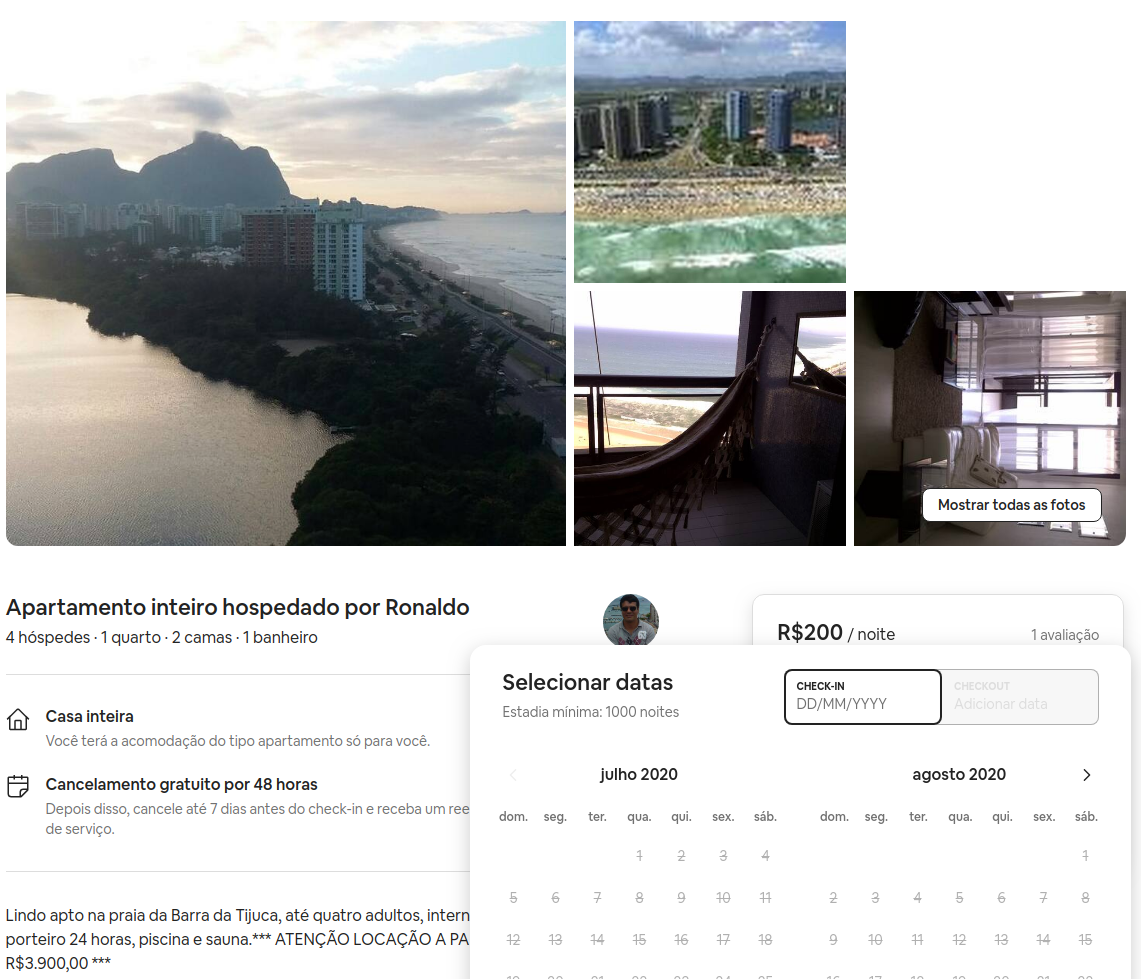
\includegraphics[width=\textwidth,height=0.5\textheight]{../fig/exemplo_periodo_airbnb.png}
\caption{Um exemplo de valor extremo de quantidade minima de
noites.\label{fig:minima_noites}}
\end{figure}

\hypertarget{apuxeandice-b}{%
\chapter*{APÊNDICE B}\label{apuxeandice-b}}
\addcontentsline{toc}{chapter}{APÊNDICE B}

O algoritmo abaixo realiza a otimização dos hiperparâmetros do Random
Forest.

\begin{algorithm}[H]
  \KwData{Base de Treino}
  \KwResult{Hiperparâmetros com menor erro}

  \SetKwProg{Pn}{Fun\c{c}ão}{:}{\Return erro}
      \Pn{TestaHiperparametros(folds, [hiperparâmetros])}{

        erro = [] \;

         \Para{i = 1 \textbf{ at\'{e} } 10}{
            train = PegaPartesdeTreino(folds, i)

            test = PegaPartedeTeste(folds, i)

            model = RandomForest(train, [hiperparâmetros])

            erro.append(EQM(model, test))
        }
    }

  folds = Separar a base em 10 partes para validação cruzada

  \Para{i = 1 \textbf{ at\'{e} } T}{
    \nosemic amostra = Gera uma amostra aleatória com 10 hiperparâmetros não testados

    TestaHiperparametros(folds, amostra)

    modelo = RandomForest(Hiperpar\^ametros testados, erro \sim hiperpar\^ametros)

    previsão = Prevê o valor do erro dos hiperpar\^ametros não testados

    amostra = Avalia o top 10 com menor previsão de erro

    TestaHiperparametros(folds, amostra)
  }

\caption{Algoritmo para encontrar um bom conjunto de hiperparâmetros}
\label{alg:hiper}
\end{algorithm}

\backmatter
\end{document}
